\documentclass[12pt]{article}

\usepackage{graphicx} % For including graphics
\usepackage{titling} % For customizing the title section
\usepackage{color}
\usepackage[margin=1in]{geometry} % For page margins
\usepackage{graphicx} % For including graphics
\usepackage[colorlinks=true, allcolors=blue]{hyperref}
\usepackage{graphicx} % For including graphics
\usepackage{hyperref} % For hyperlinks in the table of contents
\usepackage{amsmath} % For mathematical formulas
\usepackage{listings} % For code listings
\usepackage{xcolor} % For coloring code
\usepackage{amsfonts} % For mathematical fonts
\usepackage{amssymb} % For mathematical symbols
\usepackage[utf8]{inputenc}
\usepackage[margin=1in]{geometry}
\usepackage{bm}
\usepackage[style=numeric, sorting=none, sortcites=true]{biblatex}
\usepackage{appendix}
\usepackage{booktabs}
\usepackage[section]{placeins}



\addbibresource{citations.bib}


% Your title here
\title{Disaster Route Planning}
\author{} % Empty author to remove it from title area
\date{} % Empty date to remove it from title area

% Begin Document
\begin{document}

% Title Page
\begin{titlepage}
    \centering
    \vspace*{1 cm}
    \textbf{\Large Disaster Route Planning in Montreal}\\[2 cm] % Title of your document
    
\includegraphics[scale=0.5]{mcgill_logo.png}\\[1 cm] % Replace with your college logo
    \textbf{Group 3:}\\[0.5 cm]
    Arnav G. -- 260658711\\
    Lakshya A. -- 261149449\\
    Michael M. -- 261060598\\
    Nandani Y. -- 261137002\\
    Om S. -- 261112933\\[1 cm]
    \textbf{MGSC 662 Decision Analytics}\\[0.5 cm]
    Professor Javad Nasiry\\[1 cm]
    \textbf{Desautels Faculty of Management}\\
    \textbf{McGill University}\\[2 cm]
    \textcolor{red}{\hrulefill}\\[0.5 cm]
\end{titlepage}


% Table of Contents
\tableofcontents
\newpage


% Introduction
\section{Introduction}
Disasters, both natural and man-made, pose a significant challenge in urban areas, necessitating effective planning and rapid response strategies. This project introduces an advanced optimization system focused on enhancing disaster response through intelligent route planning for bus-based evacuations. In the face of emergencies, traditional transit systems often become disrupted, emphasizing the need for efficient, adaptable evacuation operations.

The significance of disaster planning cannot be understated, especially in densely populated urban environments. Effective disaster response requires not only immediate action but also strategic foresight and planning. In many cities, the existing infrastructure, while robust under normal circumstances, may not be equipped to handle the sudden and intense demands of a disaster scenario. This creates a critical need for systems that are capable of anticipating and adapting to the evolving nature of emergencies.

In this study, the dynamic and unpredictable challenges of disaster response are addressed with a focus on optimizing transportation logistics. Developing a system that can adapt in real-time to the changing requirements of a disaster situation is crucial. Montreal, with its dense population and intricate transit network, exemplifies an urban landscape where efficient disaster response is vital. The proposed system in this project aims to utilize the city's existing transit infrastructure effectively while introducing flexible measures to ensure rapid and safe evacuation during times of crisis.

This project's exploration into route optimization for disaster evacuations in Montreal offers insights into the broader field of urban disaster response. It presents a model that can be instrumental in improving evacuation strategies, ultimately contributing to the safety and well-being of urban populations in times of crisis.

\section{Problem Description and Formulation}

\subsection{Context}

In Montreal, the optimization of evacuation routes takes on added complexity due to the potential for diverse disaster scenarios. The city's layout presents a unique set of challenges, where traditional transit solutions may fall short during emergencies. This project aims to address these complexities by developing a routing model that is not only efficient in normal conditions but also highly adaptable in emergency situations. The goal is to ensure that evacuation planning is robust, responsive, and capable of handling the sudden shifts in transit dynamics that disasters often bring.

\subsection{Methodology}
To address the challenges of disaster response in urban areas, this project proposes a model that optimizes evacuation routes for a fleet of buses.
In the academic literature, this is known as the \textit{Vehicle Routing Problem} (VRP), which is a generalization of the \textit{Traveling Salesman Problem} (TSP).
The VRP is a combinatorial optimization problem that seeks to identify the optimal set of routes for a fleet of vehicles tasked with servicing a set of demand nodes.


In this section, we outline the construction of the Capacitated Vehicle Routing Problem (CVRP) model aimed at optimizing disaster evacuation routes.
The model seeks to identify the shortest possible routes for a fleet of buses tasked with evacuating residents to designated shelters, taking into account the constraints imposed by potential disaster scenarios that affect the city's transit network.

After the CVRP is formulated, we introduce a series of algorithms to convert the problem into a Split Delivery Vehicle Routing Problem (SD-VRP) \cite{DROR1994239}.
In a SD-VRP, a demand node may have capacity requirements that exceed the capacity of a single vehicle.
This necessitates formulating a problem that allows for that demand node to be visited by more than one vehicle.


\subsubsection{Data Collection and Preparation}

A comprehensive data collection forms the foundation of the Vehicle Routing Problem (VRP) model.
We utilized the General Transit Feed Specification (GTFS) from \href{https://www.stm.info/en/about/developers}{Société de transport de Montréal} for detailed transit routes, schedules, and stop information.
After the requisite data was collected, a random sample of bus stops can be taken. Then, a user-defined depot can be added to the sample of stops.

Additionally, road distances between all nodes were obtained via the OSMnx\cite{BOEING2017126} package, providing information on the actual travel distances within the city's road network.
This integration of OSMnx data ensures that the model's distance calculations are approximately true to the real-world distances.
The collected data was cleaned and preprocessed to ensure compatibility with the modeling environment and to establish a reliable baseline for the optimization process.

\subsection{Mathematical formulation of CVRP} \label{sec:cvrp}

The CVRP model is formulated as follows:
\subsubsection{Parameters}\label{sec:parameters}
Formally, the parameters to the model are defined as:
\begin{itemize}
    \item The set of all stops is defined as $S = \{0, 1, 2, ..., n\}$, where $n$ is the number of stops. The depot is defined as the node ${0}$.
    \item The set of disaster-stops is defined as $O = \{1, 2, ..., m\}$, where $m$ is the number of stops.
    \item The set of serviceable stops is then defined as $V = S - O$, i.e, the set of all stops excluding the disaster-stops.
    \item The distance between two nodes $i$ and $j$ is denoted as $D_{ij}$ and is assumed to be symmetric, i.e., $D_{ij} = D_{ji}$.
    \item The demand at node $i, \forall i \in V - \{0\}$ is denoted as $q_i \sim U(L, H)$,
          where $L$ and $H$ are the lower and upper bounds of the uniform distribution, respectively.
    \item The capacity of each bus is denoted as $Q$
    \item The number of buses is denoted as $K$
    \item The distance threshold between any two non-depot nodes is denoted as $D_{max}$

\end{itemize}

\subsubsection{Assumptions}
\begin{itemize}
    \item Stable and Predictable Road Network: The model assumes that the road network remains stable and predictable during a disaster. This includes the assumption that roads are passable and distances between nodes (bus stops) do not significantly change due to the disaster.
    \item Consistent Bus Capacity and Availability: The assumption here is that the capacity of each bus in the fleet is consistent and that a sufficient number of buses are available for the evacuation effort.
    \item Bus Stops as Dual-Function Points (Pick-up and Drop-off): The model assumes that bus stops function as both pick-up and drop-off points during the evacuation process. This means that each bus stop is not only used for boarding passengers but also for disembarking them at safe locations or shelters.
    \item Known Demand at each node before the bus arrives: This implies that the number of people requiring evacuation at each node is either known or can be estimated within a certain range.
\end{itemize}



\subsubsection{Decision Variables}
The decision variables to the model are defined as:
\begin{align*}
    x_{ijk} & = \begin{cases}
                    1 & \text{if the bus $k$ travels from node $i$ to node $j$} \\
                    0 & \text{otherwise}
                \end{cases} \\
    u_i     & = \text{the amount of demand satisfied at node $i$}
\end{align*}

\subsubsection{Formulation}
With the given parameters and decision variables, the model is given by:
\numberwithin{equation}{section}
\begin{alignat}{4}
     & \text{minimize:}   &       & \sum_{i=0}^{n} \sum_{j=0}^{n} \sum_{k=0}^{K} D_{ij} x_{ijk}                                                              \\
     & \text{subject to:} & \quad & \sum_{j=0}^{n} x_{ijk} = \sum_{j=0}^{n} x_{jik},            & \quad \forall i \in V, \forall k \in K                     \\
     &                    & \quad & \sum_{i=1}^{n} \sum_{k=0}^K x_{ijk} = 1,                    & \quad \forall j \in V - \{0\}                              \\
     &                    & \quad & \sum_{j=1}^{n} x_{0jk} \leq 1,                              & \quad \forall k \in K                                      \\
     &                    & \quad & \sum_{j=1}^{n} \sum_{i=0}^{n} q_j \cdot x_{ijk} \leq Q,     & \quad \forall k \in K                                      \\
     &                    & \quad & x_{iik} = 0,                                                & \quad \forall i \in V, \forall k \in K                     \\
     &                    & \quad & u_j - u_i \geq q_j - Q \cdot (1 - x_{ijk}),                 & \quad \forall i,j \in V - \{0\}, i \neq j, \forall k \in K \\
     &                    & \quad & q_i \leq u_i \leq Q,                                        & \quad \forall i \in V - \{0\}                              \\
     &                    & \quad & D_{ij} \cdot x_{ijk} \leq D_{max},                          & \quad \forall i,j \in V - \{0\}, \forall k \in K           \\
     &                    & \quad & x_{ijk} \in \{0,1\},                                        & \quad \forall i,j \in V, \forall k \in K                   \\
     &                    & \quad & u_i \in \mathbb{Z},                                         & \quad \forall i \in V
\end{alignat}

The objective function (2.1) minimizes the total distance traveled by all buses. Constraints (2.2) ensures that each bus leaves a node that it enters,
(2.3) ensures that each node is visited only once,
(2.4) ensures that each bus leaves the depot at most once,
(2.5) ensures that the capacity of each bus is not exceeded,
and (2.6) ensures that a bus does not travel from a node to itself.


Constraints (2.7) and (2.8) are the Miller-Tucker-Zemlin (MTZ) constraints to eliminate subtours,
i.e., cycling routes that do not pass through the depot.

Constraints (2.9) impose a distance restriction of $D_{max}$ on travel between any two non-depot nodes.
This is to ensure that the model does not generate routes that are infeasible in the real world.

Constraints (2.10) and (2.11) define the decision variables as binary and integer, respectively.

\subsection{Split Delivery VRP}
In the above formulation, the demand at each node is assumed to be less than or equal to the capacity of a single bus.
If the demand at node $i$ exceeds the bus capacity $Q$, then the CVRP model (defined in ~\autoref{sec:cvrp}) will not be able to produce a feasible solution.

To address this, we introduce a series of algorithms to convert the CVRP into a Split Delivery VRP (SD-VRP).

The idea is to split the each node with $q_i > Q$ into multiple nodes of smaller demands. The choice of the algorithm to split a node impacts the scale of the problem, and hence the computational time required to solve it.

\subsubsection{Geometric split}
This method splits a node's demand $q_i$ according to the following geometric progression:
\begin{equation}
    q_{ix} = \frac{2^{x-1}}{\sum_{i=1}^{S} 2^{x-1}} q_{i} \quad \forall x \in \{1, 2, ..., S\}
\end{equation}
$q_{ix}$ is rounded down to the nearest integer. If $\sum_{i=1}^{S} q_{ix} < q_{i}$, then $q_{iS} = q_{iS} + (q_{i} - \sum_{i=1}^{S} q_{ix})$.

\subsubsection{Capacity-based split}
This method splits a node's demand $q_i$ into $S$ nodes of equal demand:
\begin{equation}
    q_{ix} = Q  \quad \forall x \in \{1, \dots, S = \frac{q_{i}}{Q}\} \\
\end{equation}
$q_{ix}$ is rounded down to the nearest integer. If $\sum_{i=1}^{S} q_{ix} < q_{i}$, then $q_{i(S+1)} = q_{i} - \sum_{i=1}^{S} q_{ix}$.

\subsubsection{Random split}
This method splits a node's demand $q_i$ into $S$ nodes of random demand:
\begin{equation}
    q_{ix} \sim U(1, Q) \quad \forall x \in \{1, \dots, S = \frac{q_{i}}{Q}\}, \quad q_{ix} \in \mathbb{Z}^+\\
\end{equation}

\subsubsection{Equal split}
This method splits a node's demand $q_i$ into $S$ nodes of equal demand of 1:
\begin{equation}
    q_{ix} = 1 \quad \forall x \in \{1, \dots, S = q_{i}\} \\
\end{equation}

\subsubsection{Comparison of split methods}
Given a node with demand $q_n = 97$ and a bus capacity of $Q = 75$, ~\autoref{tab:split-methods} compares the different split methods.
We report the number of nodes generated by each method, and the demand at each node.

From \autoref{tab:split-methods}, we see that the equal split method provides the highest flexibility for the model by splitting each node into its smallest possible demand. However, this comes at the cost of a large number of nodes, which increases the computational time required to solve the model.

The geometric split method provides a good balance between the number of nodes and the demand at each node, and hence is the method we use in our model, however the model can be easily modified to use any of the other split methods.

\begin{table}[htbp]
    \centering
    \begin{tabular}{|c|c|c|c|}
        \hline
        \textbf{Split Method} & \textbf{Number of Nodes} & \textbf{Node Demands}   \\
        \hline
        Geometric Split       & 6                        & $[1, 3, 6, 12, 24, 51]$ \\
        \hline
        Capacity-based Split  & 2                        & $[75, 22]$              \\
        \hline
        Random Split          & 3                        & $[12, 74, 11]$          \\
        \hline
        Equal Split           & 97                       & $[1, 1, ..., 1]$        \\
        \hline
    \end{tabular}
    \caption{Comparison of Split Methods}
    \label{tab:split-methods}
\end{table}

\newpage
\section{Numerical implementation \& results}
This section presents the numerical implementation of the SD-VRP model, and the results obtained from the models.
The models were implemented in Python using the Gurobi solver.

\subsection{Model parameters}
The parameters used in the model are given in ~\nameref{sec:parameters}. For this particular example, we assume that:
\begin{itemize}
    \item The number of buses, $K = 20$
    \item The bus capacity, $Q = 100$
    \item The number of stops (inclduing depot), $n = 31$
    \item The number of disaster stops, $m = 4$
    \item The lower bound of the demand distribution, $L = 1$
    \item The upper bound of the demand distribution, $H = 140$
    \item The distance threshold between any two non-depot nodes, $D_{max} = 7$
\end{itemize}

Then, the demand at each node is generated as $q_i \sim U(L, H)$, where $L$ and $H$ are the lower and upper bounds of the uniform distribution, respectively.

Further, we assume the following parameters for the Gurobi solver, namely:
\begin{itemize}
    \item \texttt{TimeLimit} = 15 * 60 = 900 seconds
    \item \texttt{MIPGap} = 0.1
    \item \texttt{MIPFocus}\footnote{\href{https://www.gurobi.com/documentation/current/refman/mipfocus.html}{MIPFocus - Gurobi Documentation}} = 1
\end{itemize}

Adding a depot at McGill University and choosing a disaster-affected area, the unsolved network is shown in ~\autoref{fig:unsolved-network}.
Based on the generated demand, 6 nodes exceeded the bus capacity $Q$.

We then solve the model using three split methods\footnote{The equal split method takes a long time to compute, and therefore, has been omitted from this example}, namely:
\begin{enumerate}
    \item Geometric split
    \item Capacity-based split
    \item Random split
\end{enumerate}

\subsection{Results}
The results obtained from the model for each type of split method are summarized below:

\begin{table}[htbp]
    \centering
    \begin{tabular}{|c|c|c|c|}
        \hline
        \textbf{Split Method}            & \textbf{Geometric Split}         & \textbf{Capacity-based Split}   & \textbf{Random Split}         \\
        \hline
        \textbf{Total number of nodes}   & 54                               & 32                              & 36                            \\
        \hline
        \textbf{Total distance (in kms)} & 199.10                           & 198.26                          & 200.04                        \\
        \hline
        \textbf{Number of buses used}    & 16                               & 16                              & 16                            \\
        \hline
        \textbf{Time taken (in seconds)} & 900                              & 900                             & 900                           \\
        \hline
        \textbf{MIPGap}                  & 81.55\%                          & 23.98\%                         & 41.20\%                       \\
        \hline
        \textbf{Route map}               & ~\autoref{fig:geometric-network} & ~\autoref{fig:capacity-network} & ~\autoref{fig:random-network} \\
        \hline
    \end{tabular}
    \caption{Results for the SD-VRP model}
    \label{tab:results}
\end{table}

The route map for each split method shows the routes taken by each bus.
The color of the route indicates the bus number.
Nodes in red indicate disaster-affected areas,
and nodes in purple indicate nodes with demand greater than the bus capacity.

\subsection{Discussion and Understanding}
From ~\autoref{tab:results}, we see that
the capacity-based split method provides the best results in terms of the total number of nodes, total distance, and time taken to solve the model.

Other simulations can be run by varying the parameters of the model to obtain a better understanding of the trade-offs between the different split methods.

The outcomes of the model are coherent and align with established benchmarks in Capacitated Vehicle Routing Problem (CVRP) research globally (refer to ~\autoref{fig:google-cvrp} for a CVRP solution diagram from Google's OR-Tools, which is similar to our solution).

An examination of the route maps corroborates the model's efficacy, as it demonstrates that buses systematically return to the depot upon reaching their capacity limits (see ~\autoref{tab:load-table-geometric} for the load accumulation table for each bus).

Furthermore, the model exhibits an innate intelligence in managing the complexity of the routes, avoiding the creation of subtours and effectively addressing the demands at disaster-affected nodes. This clustering effect, which organically emerges from the model's design, is a hallmark of an optimized CVRP solution, reflecting a sophisticated understanding of routing dynamics.

The data also reveal the model's proficiency in handling situations where the demand at certain nodes surpasses the bus capacity. The resulting routes and network diagrams, which can be found in the designated appendices, indicate that these nodes are adequately divided and assimilated into the final routing scheme.

It is particularly noteworthy that the model accommodates scenarios wherein split nodes are serviced by different buses, suggesting a level of complexity where the optimal path diverges based on the chosen split strategy. This not only underscores the model's adaptability but also its strategic depth in calculating efficient pathways (see ~\autoref{route:geometric-route} for route prints and ~\autoref{route:geometric-network-plot} for network diagram).

Overall, the solution not only meets the theoretical expectations of CVRP problems but also displays an impressive level of practical sophistication and real-world applicability. The results reflect a robust and well-engineered system capable of delivering efficient disaster response routes within the demanding constraints of urban scenarios.


\newpage

\section{Problem Extensions}
\subsection{Safe Zones}

In our extended model addressing disaster response logistics, we introduce the concept of "Safe Zones" and the incorporation of nearest bus stops to disaster areas. This modification is crucial in scenarios where direct access to the disaster area is not possible. In such cases, individuals in the disaster area are assumed to move to the nearest accessible bus stop, effectively transferring the demand from the disaster area to these nearest stops. Buses then transport these evacuees from these "nearest stops" collection points to designated Safe Zones. For our model, we consider specific locations such as the Bell Centre and Olympic Stadium as Safe Zones.

To facilitate this, we introduce a new set $N = \{n_1, n_2, \ldots, n_r\}$ representing the nearest bus stops to the disaster area. Additionally, we define a binary decision variable $y_{nk}$ for each bus $k \in K$ and nearest stop $n \in N$, indicating whether bus $k$ visits nearest stop $n$.

The routing constraint is redefined as follows to ensure that buses visiting a stop in $N$ also visit at least one Safe Zone:

$$
    \sum_{n \in N} y_{nk} \leq \sum_{z \in Z} x_{znk} \quad \forall k \in K
$$

In this constraint, $Z$ represents the set of Safe Zones, and $x_{znk}$ is a binary variable indicating if bus $k$ travels from stop $n$ to Safe Zone $z$. This constraint ensures that if a bus visits a stop near the disaster area, it must also visit a Safe Zone.

Our optimization process considering these constraints yielded the following results\footnote{$\Delta$ represents change from ~\autoref{tab:results}}:

\begin{table}[htbp]
    \centering
    \begin{tabular}{|c|c|c|c|c|c|c|}
        \hline
        \textbf{Split Method} & \textbf{Geometric} & \textbf{$\Delta$ } & \textbf{Capacity} & \textbf{$\Delta$ } & \textbf{Random} & \textbf{$\Delta$ } \\
        \hline
        Total number of nodes & 55                 & 1                  & 33                & 1                  & 37              & 1                  \\
        \hline
        Total distance (kms)  & 207.90             & 8.80               & 200.04            & 1.78               & 205.76          & 5.72               \\
        \hline
        \# of buses used      & 16                 & -                  & 16                & -                  & 17              & 1                  \\
        \hline
        Time taken (s)        & 900                & -                  & 900               & -                  & 900             & -                  \\
        \hline
        MIPGap                & 79.07\%            & -2.48pp            & 20.43\%           & -3.55pp            & 28.16\%         & -13.04pp           \\
        \hline
    \end{tabular}
    \caption{Results for the Safe Zone Problem Extension}
    \label{tab:results-extension}
\end{table}

The analysis of different split methods in our extended disaster response logistics model reveals noteworthy insights. The geometric split, with its highest node count and total distance, indicates a more intricate routing structure, possibly due to the distributed nature of geometric splitting.

In stark contrast, the capacity-based split emerges as remarkably efficient, which makes it an attractive option for scenarios demanding rapid decision-making, despite its marginally longer total distance.

The random split, while slightly less efficient in terms of distance compared to the geometric split, does not deviate excessively, suggesting a moderate trade-off between randomness and structured planning. A critical observation across all methods is the consistency in bus utilization, implying that the current fleet size is well-suited for varying operational strategies.

The substantial difference in the Model Integration and Programming (MIP) Gap, especially the higher gap observed in the geometric split, indicates varying degrees of solution optimality and might necessitate additional computational resources or time for more refined results. These findings not only enhance our understanding of evacuation logistics in disaster scenarios but also underscore the importance of method selection based on specific operational goals and constraints. Looking forward, this analysis opens avenues for exploring hybrid split methods, incorporating real-time data for dynamic routing, and including additional logistical considerations unique to emergency scenarios, thereby contributing to the evolution of more robust and responsive disaster management strategies.

\subsection{Minimize Bus Travel Time}

The original problem focused on minimizing the total distance traveled during disaster evacuations. However, in a real-world scenario, especially during a disaster, time becomes a more critical factor. We can also explore another extension in the future where we aim to minimize the total time taken for evacuation, incorporating real-time traffic flow data to estimate travel times more accurately.

For this, we can integrate real-time traffic data from sources like Google Maps, Waze, and local traffic systems. This data helps adjust evacuation routes based on traffic conditions, road closures, and accidents. Additionally, integrating weather forecasts, public transport updates, and emergency services data enhances our ability to plan and adapt evacuations during disasters.

The new objective function will hence aim to minimize the total time taken for evacuation. The time taken to travel between two nodes i and j is denoted as $T_{ij}$, which is a function of the distance $D_{ij}$ and the average speed $V_{ij}$ based on real-time traffic data.

\begin{alignat}{4}
     & \text{minimize:}                &       & \sum_{i=0}^{n} \sum_{j=0}^{n} \sum_{k=0}^{K} T_{ij} x_{ijk}                                               \\
     & \text{additionally subject to:} & \quad & T_{ij} = \frac{D_{ij}}{V_{ij}(t)},                          & \quad \forall i,j \in V, \forall t \in Time \\
     &                                 & \quad & \sum_{i=1}^{n} \sum_{j=1}^{n} T_{ij} x_{ijk} \leq T_{max},  & \quad \forall k \in K
\end{alignat}

The objective function (4.1) minimize the total time taken by all buses to visit every node. Constraints (4.2) take the distance between two nodes $D_{ij}$ and the average speed $V_{ij}$ to calculate the time taken $T_{ij}$. Constraints (4.3) impose a time limit on travel between two non-depot nodes.

By integrating real-time data and focusing on time minimization, the model becomes more dynamic and adaptable to the ever-changing conditions of an urban disaster scenario. This approach enhances the effectiveness of disaster evacuation planning, leading to safer and more efficient evacuations.




\newpage
\section{Recommendations and Conclusions}

The paper presented a comprehensive Split Delivery Vehicle Routing Problem (SD-VRP) model designed to optimize bus routes for emergency evacuations in Montreal. The primary objective is to minimize total distance, which is crucial for enhancing disaster response efficiency and reducing human suffering during emergencies.

In the realm of the business value proposition, this formulation offers remarkable flexibility. It transcends the confines of specific disaster types by enabling us to dynamically customize affected areas. This adaptability positions us to cater to a wide-ranging market audience, spanning from local government agencies responsible for public safety and emergency management, to disaster response organizations, including NGOs and relief agencies. Moreover, it proves indispensable for urban planners and developers dedicated to crafting resilient urban infrastructures, as well as technology integrators specializing in innovative smart city solutions.

As a consultant, the following recommendations are proposed for future development:
\begin{itemize}
    \item \textbf{Stakeholder Collaboration:} Engaging with local authorities, emergency services, and urban planners is essential. Their feedback will refine the model, making it more effective in real-world scenarios.

    \item \textbf{Real-Time Data Integration:} Incorporating real-time traffic and weather data will allow for dynamic rerouting during disasters, enhancing the model's effectiveness.

    \item \textbf{Model Scalability and Flexibility:} Testing and enhancing the model for different urban layouts and disaster scenarios is crucial. This includes adaptation for cities with varying transit systems and population densities.

    \item \textbf{User-Friendly Interface:} Developing an intuitive interface will make the model accessible to a broader range of users, facilitating faster decision-making during emergencies.

    \item \textbf{Simulation and Training:} Regular drills with emergency responders using the model can identify potential issues and areas for improvement in evacuation processes.
\end{itemize}
\subsection{Key Learnings}
The project highlighted the complexities of disaster management and SD-VRP, especially when demand exceeds vehicle capacity. Employing heuristics for node splitting was challenging, and finding optimal solutions remains a key focus for future research. The project underscored the importance of high-quality data in modeling and the impact of urban design on disaster response. It also emphasized the need for urban planning that considers emergency response logistics.

\subsection{Improvements and Bottlenecks}
Incorporating real-time data for time optimization, such as traffic flow, will enhance the model's realism and applicability in emergency scenarios. This addition is crucial for prioritizing evacuation efforts and provides practical insights into the ethical dilemmas often encountered in disaster management.

The model currently faces scalability issues, with runtime increasing exponentially with more nodes. Addressing this through more efficient algorithms or parallel computing could be beneficial. Additionally, the reliance on static data limits adaptability; integrating live data feeds would significantly enhance the model's effectiveness in dynamic disaster scenarios.

In conclusion, while the SD-VRP model presents a significant advancement in optimizing emergency evacuations, continuous improvements and adaptations are necessary to address real-world challenges more effectively. Engaging with key stakeholders, enhancing data integration, and addressing computational challenges are essential steps towards realizing its full potential in disaster response and urban planning.

\newpage

\begin{appendices}
    \section{Appendix}
    \subsection{Figures}\label{app:figures}
    \begin{figure}[!htb]
        \centering
        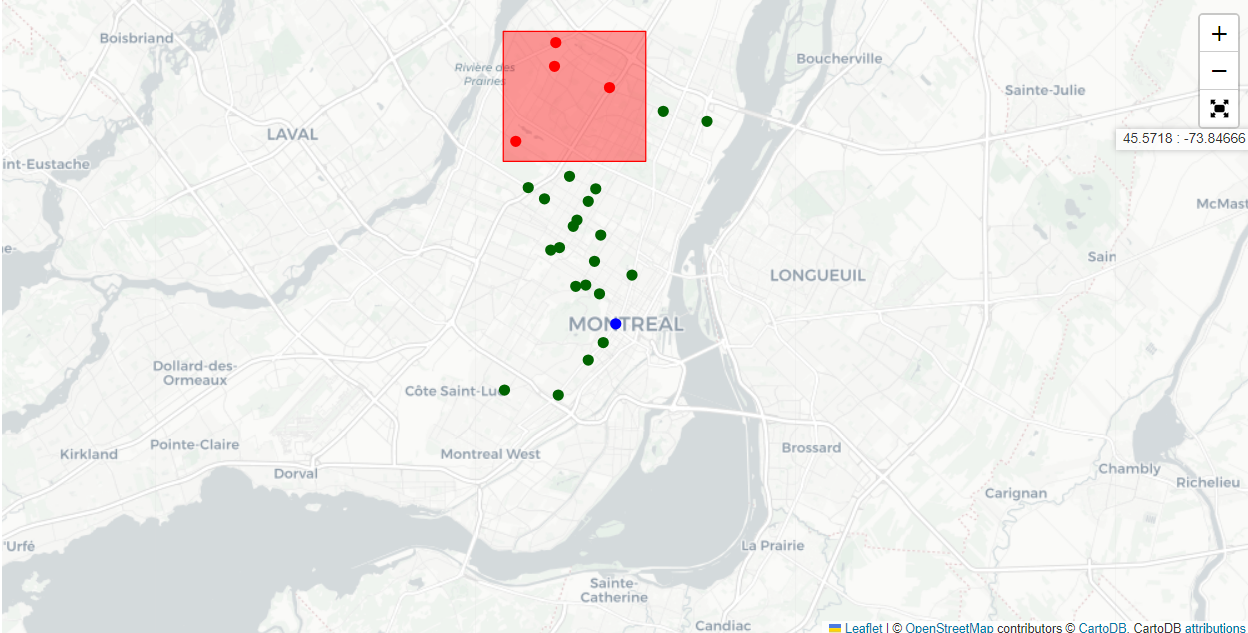
\includegraphics[width=0.6\textwidth]{unsolved-network.png}
        \caption{Unsolved Network}
        \label{fig:unsolved-network}
    \end{figure}

    \begin{figure}[!htb]
        \centering
        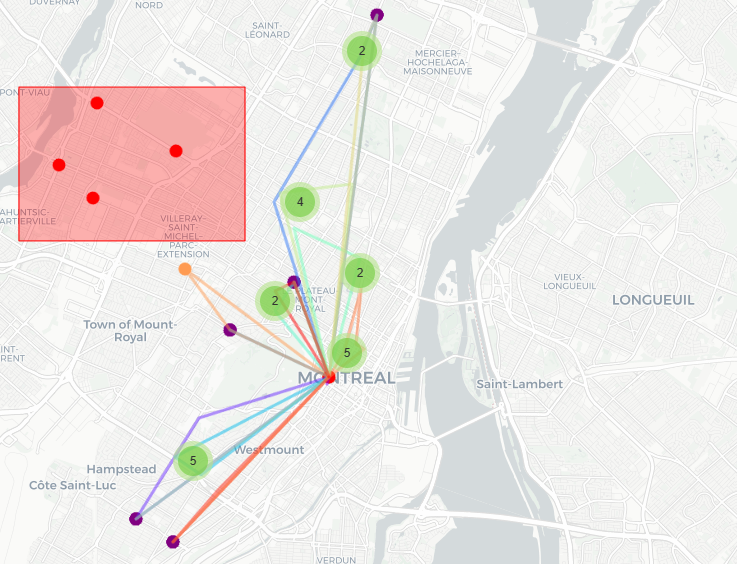
\includegraphics[width=0.6\textwidth]{geometric-network.png}
        \caption{Geometric Split Network}
        \label{fig:geometric-network}
    \end{figure}

    \begin{figure}[!htb]
        \centering
        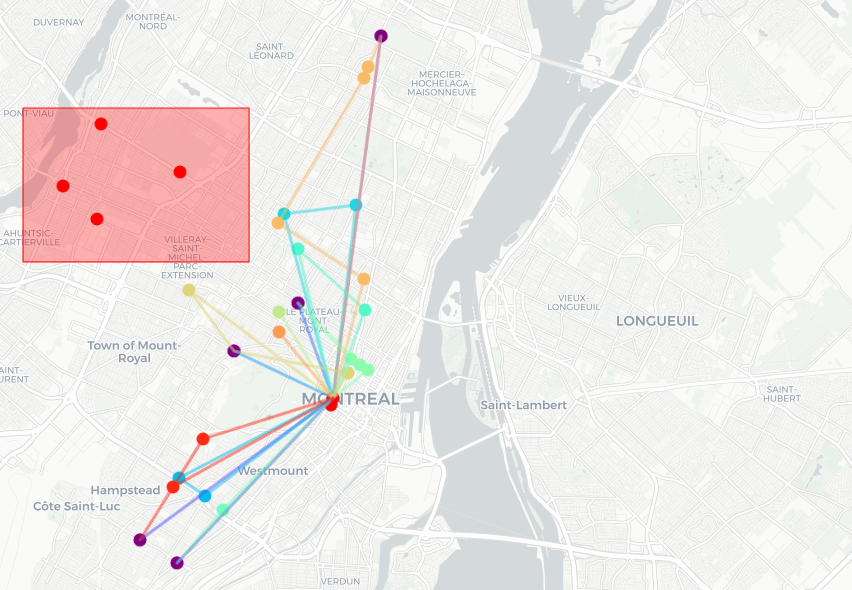
\includegraphics[width=0.6\textwidth]{capacity-network.png}
        \caption{Capacity-based Split Network}
        \label{fig:capacity-network}
    \end{figure}

    \begin{figure}[!htb]
        \centering
        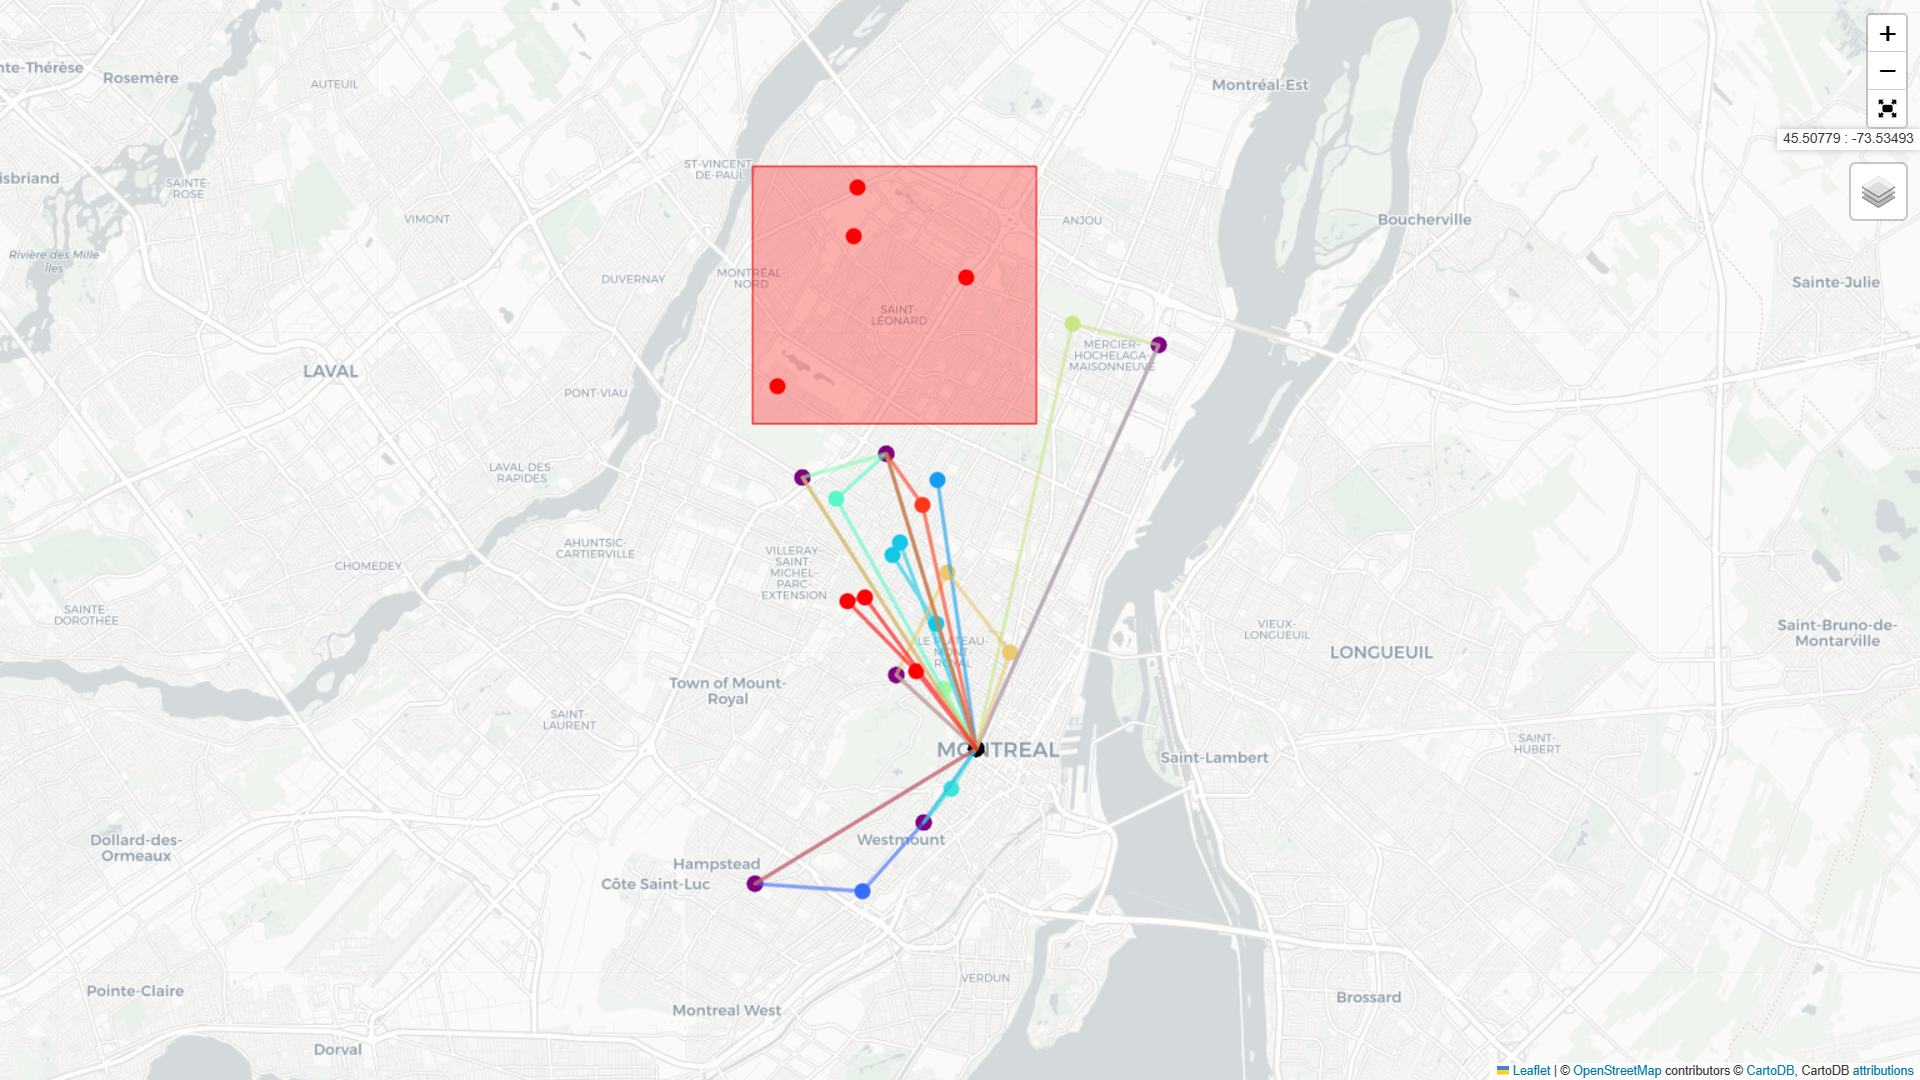
\includegraphics[width=0.6\textwidth]{random-network.png}
        \caption{Random Split Network}
        \label{fig:random-network}
    \end{figure}

    \begin{figure}[!htb]
        \centering
        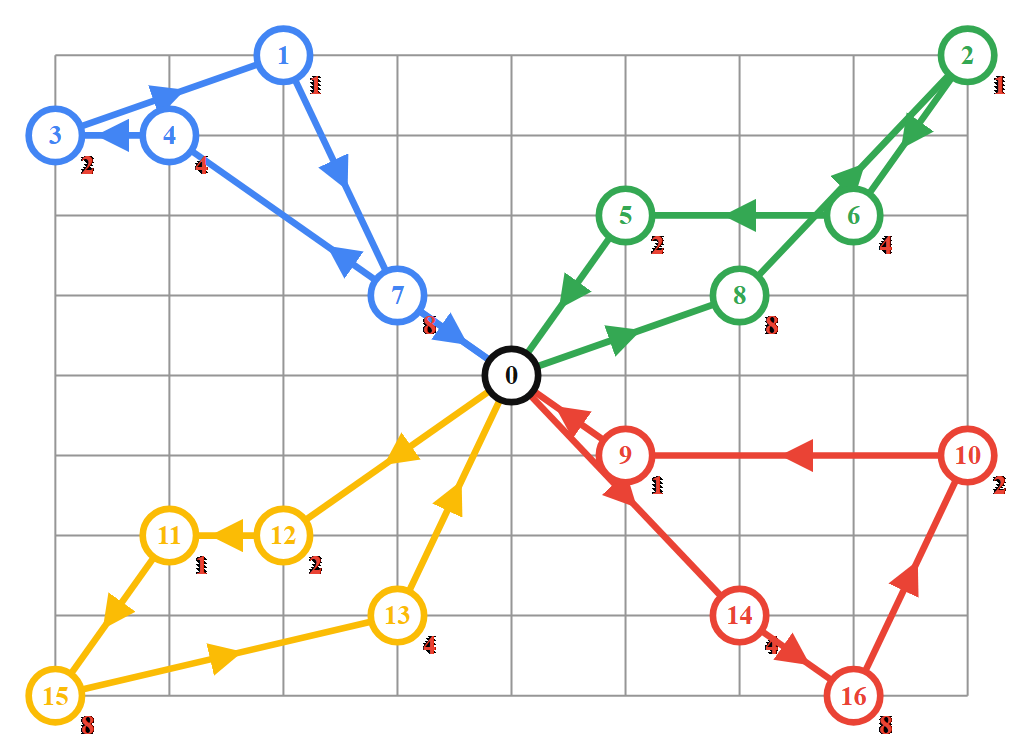
\includegraphics[width=0.6\textwidth]{google-cvrp.png}
        \caption{CVRP Solution from \href{https://developers.google.com/optimization/routing/cvrp}{OR-Tools}}
        \label{fig:google-cvrp}
    \end{figure}

    \begin{figure}[!htb]
        \centering
        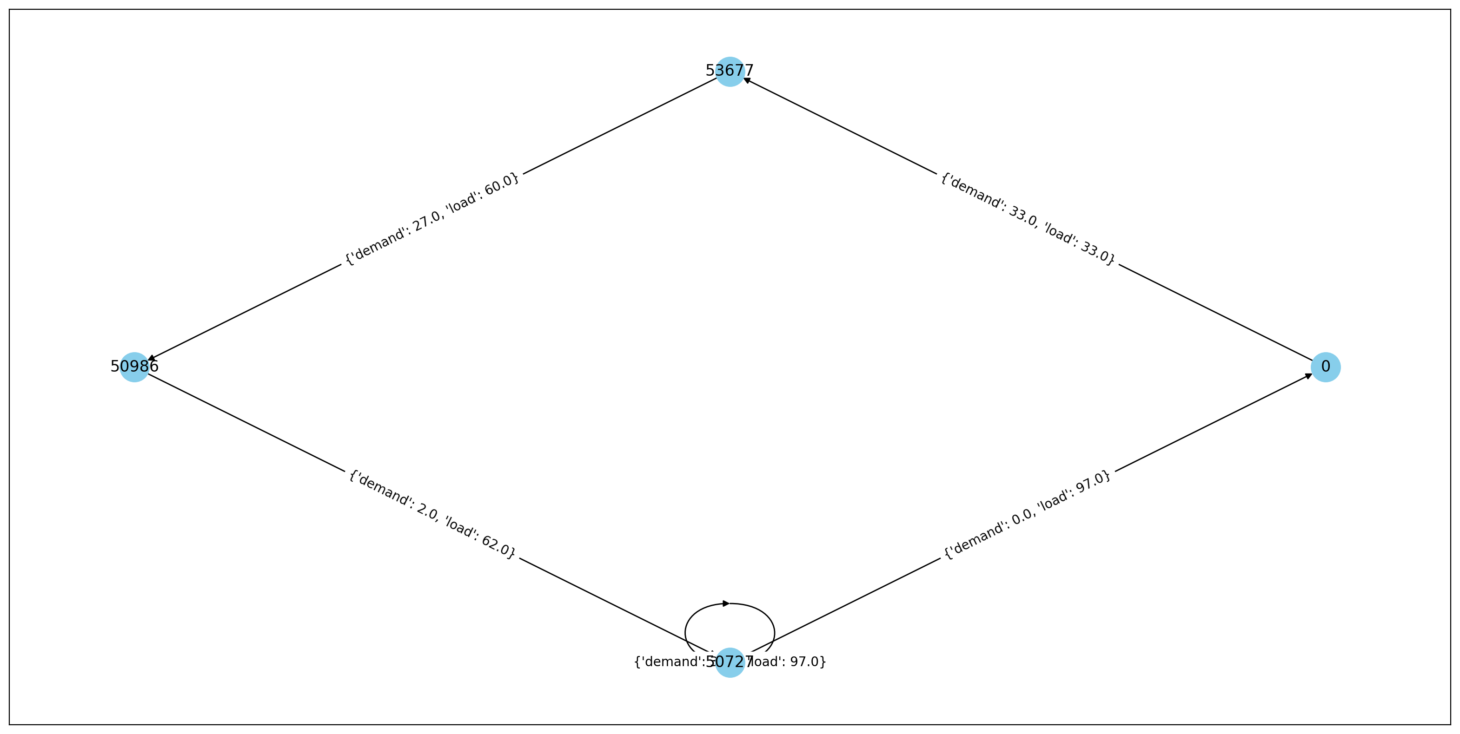
\includegraphics[width=0.6\textwidth]{geometric-network-plot.png}
        \caption{Network plot for Bus 1 - Geometric Split Network}
        \label{route:geometric-network-plot}
    \end{figure}

    \begin{figure}[!htb]
        \centering
        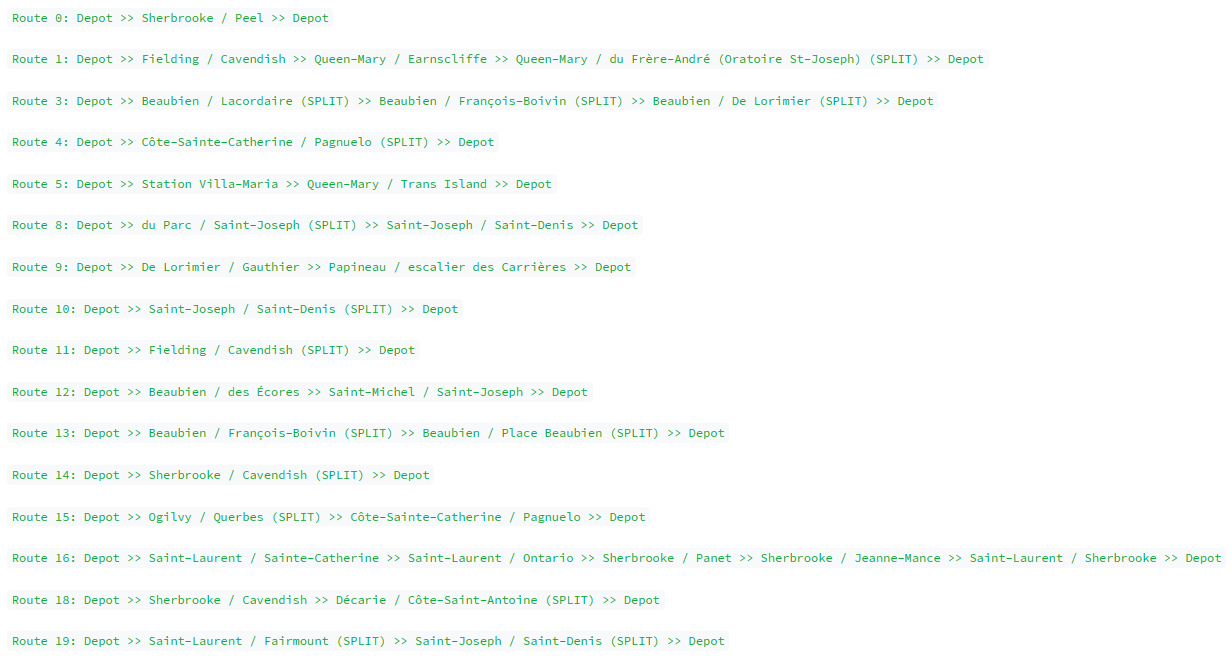
\includegraphics[width=1\textwidth]{geometric-route.png}
        \caption{Route path - Geometric Split Network}
        \label{route:geometric-route}
    \end{figure}

    \FloatBarrier
    \subsection{Tables}\label{app:routes}
    \begin{table}[!htbp]
        \centering
        \begin{tabular}{|c|c|}
            \hline
            \textbf{Bus} & \textbf{Demand} \\
            \hline
            0            & 40.0            \\
            1            & 97.0            \\
            2            & 100.0           \\
            3            & 92.0            \\
            4            & 97.0            \\
            5            & 100.0           \\
            6            & 99.0            \\
            7            & 95.0            \\
            8            & 100.0           \\
            9            & 100.0           \\
            10           & 90.0            \\
            11           & 94.0            \\
            12           & 85.0            \\
            13           & 73.0            \\
            14           & 98.0            \\
            15           & 98.0            \\
            \hline
        \end{tabular}
        \caption{Load Accumulation Table ($Q=100$)}
        \label{tab:load-table-geometric}
    \end{table}
\end{appendices}


\newpage
\printbibliography
\newpage

\end{document}
